% This example An LaTeX document showing how to use the l3proj class to
% write your report. Use pdflatex and bibtex to process the file, creating 
% a PDF file as output (there is no need to use dvips when using pdflatex).

% Modified 

\documentclass{l3proj}
\usepackage{datetime}

\begin{document}
\title{Algorithm Animator}
\author{Arthur Bigeard \\
		Alexander Ferguson \\
		Andrew Gibson \\
		Gediminas Leikus \\
		Liam Bell}
\usdate
\date{\today}
\maketitle
\begin{abstract}

For teaching purposes it is useful to be able to animate algorithms and produce a visual representation of how they work. The basic idea is to use a diagrammatic representation of a data structure, for example an array or a tree, and illustrate the algorithm step by step, showing how the data structure is accessed and changed. The aim of this project is to design and implement a system for animating algorithms. There are at least two possible approaches. One is to design and implement a simple programming language in such a way that all programs are animated while being executed. Another is to design and implement an API for animations, so that an existing program (in Java, for example) can be animated by inserting calls to your library. The system should be as general as possible in the sense of supporting a range of styles of algorithm, and should be demonstrated by producing a range of animations of standard algorithms. It would also be useful to be able to 
capture the animation in a form that can be viewed independently of your system, for example as a sequence of HTML pages or a Flash animation.

\end{abstract}
\educationalconsent
\tableofcontents
%==============================================================================
\chapter{Introduction}
\label{intro}

Alice was beginning to get very tired of sitting by her sister
on the bank and of having nothing to do: once or twice she had peeped into
the book her sister was reading, but it had no pictures or conversations in
it.

\begin{figure}
\begin{center}
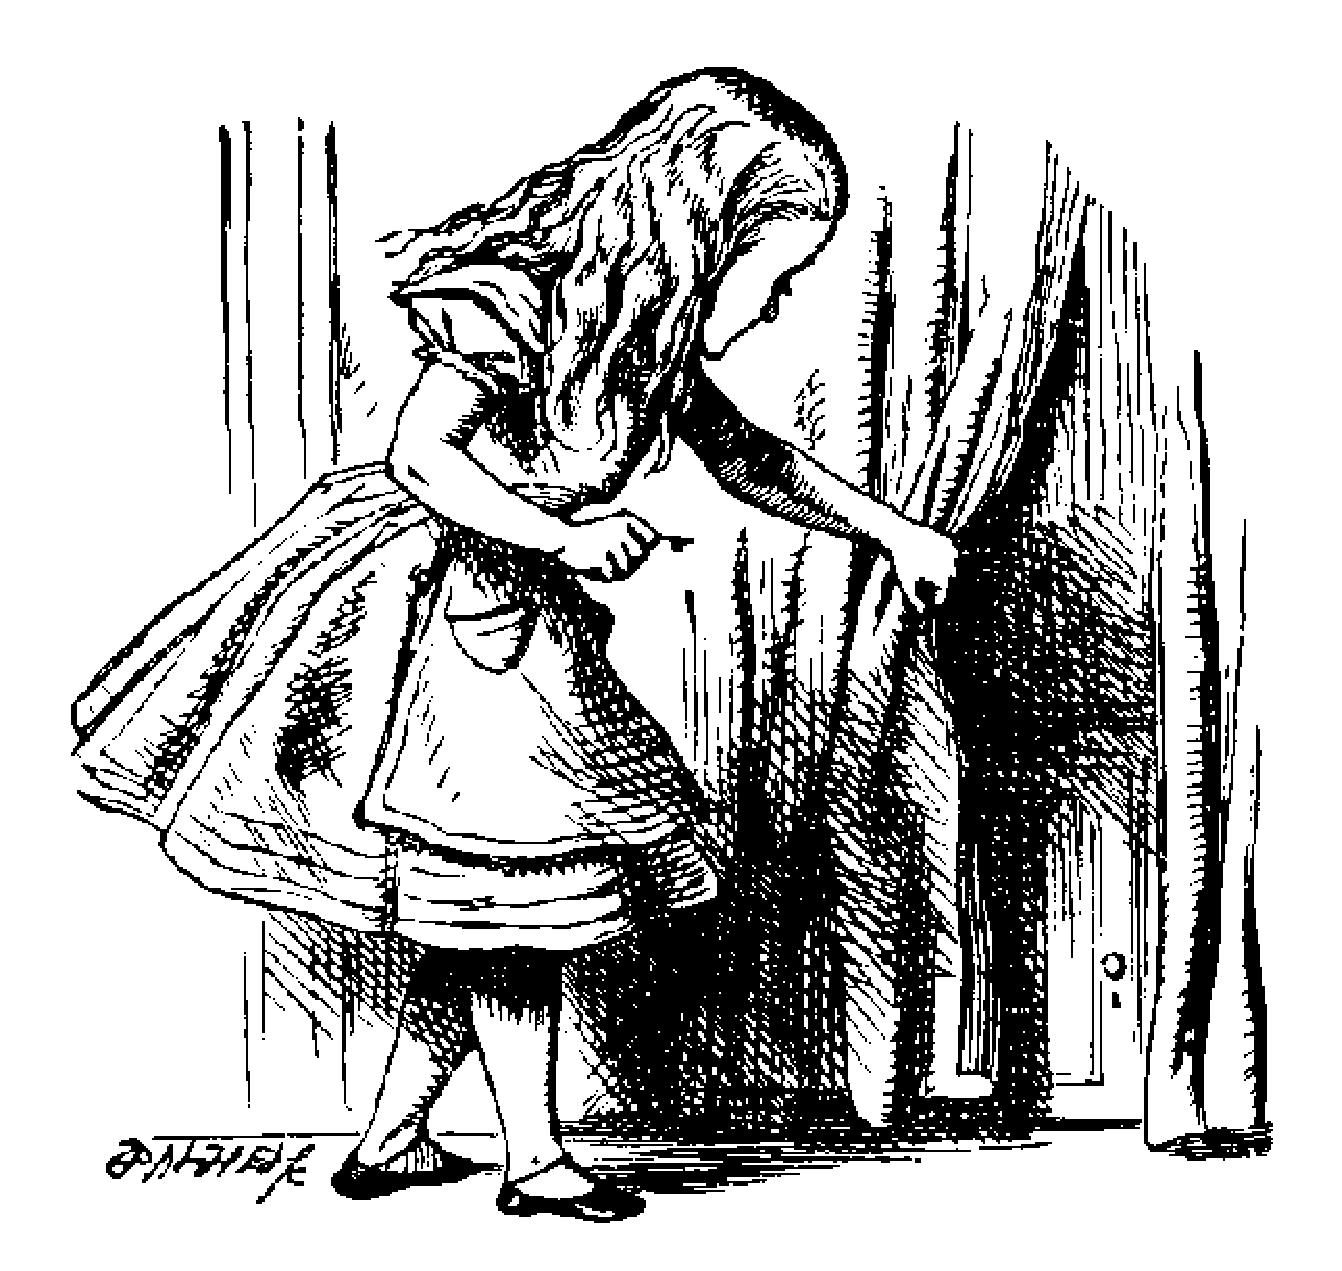
\includegraphics[width=7cm]{figures/alice}
\end{center}
\caption{Behind it was a little door}
\label{fig:alice}
\end{figure}

Alice opened the door and found that it led into a small passage, not much
larger than a rat-hole: she knelt down and looked along the passage into
the loveliest garden you ever saw.

%==============================================================================
\chapter{Design}
\label{design}

The following diagrams (especially figure) illustrate the
process...

%==============================================================================
\chapter{Implementation}
\label{impl}

In this chapter, we describe how the implemented the system.

%------------------------------------------------------------------------------
\section{User Interface}

Blah blah blah
Blah blah blah
Blah blah blah
Blah blah blah

% - - - - - - - - - - - - - - - - - - - - - - - - - - - - - - - - - - - - - - -
\section{Problems Encountered}
\subsection{Arthur Bigeard}
\subsection{Alexander Ferguson}
\subsection{Andrew Gibson}
\subsection{Gediminas Leikus}
\subsubsection{Separating animations into steps and making continuous animations}

The group decided to use Java for our project, because we were all familiar with it and because it was the language our client suggested us to use. We had left the decision of choosing the animation tools to Andrew Gibson and Alexander Ferguson. For the reasons stated in this document (reference), they decided to choose the Timing Framework \cite{website:TimingFramework}.

Andrew had an example (\ref{fig:firstPrototype}) ready, which had multiple rectangles created from an array moving back and forth, had buttons allowing us to stop the animation, resume it or delete one of the rectangles. He also added comments into the sample code, just so it would be easier for us to familiarize with the tool.

\begin{figure}
\begin{center}
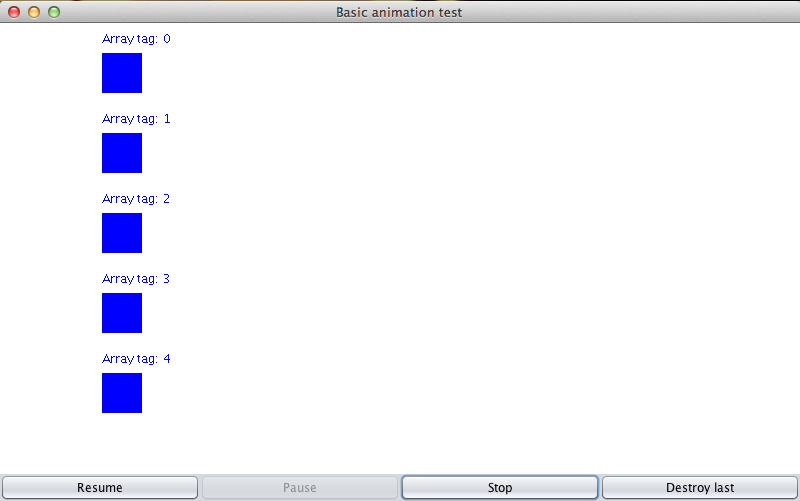
\includegraphics[width=\textwidth]{images/firstPrototype.png}
\end{center}
\caption{The first demonstration, produced by Andrew}
\label{fig:firstPrototype}
\end{figure}

While this was a good initial step, we did not have any obvious way to implement Steps, in a sense where multiple Animations could be assigned to one step and we could navigate through these steps back and forth. Therefore both Andrew and Arthur Bigeard started looking into it. \\

\begin{figure}
\begin{center}
\begin{verbatim}
public void timingEvent(Animator source, double fraction){
    boolean done = false;
    if(anArr.getToDo().size() > 0){
        Step[] steps = new Step[anArr.getToDo().peek().length];
        System.arraycopy(anArr.getToDo().peek(), 0, steps, 0, steps.length);

        for(int i = 0; i < steps.length; i++){                    
            Rectangle rect = rect_list[steps[i].getIndex()].getRec();
            double x = steps[i].getX();
            double y = steps[i].getY();
            double stepX = rect.getX();
            double stepY = rect.getY();
            if(y != stepY){
                if(Math.abs(x - stepX) < 50){
                    if(y > stepY){
                        rect_list[steps[i].getIndex()].getRec().x += 1;
                    }
                    else{
                        rect_list[steps[i].getIndex()].getRec().x -= 1;
                    }
                }
                else{
                    if(y > stepY){
                        rect_list[steps[i].getIndex()].getRec().y += 1;
                    }
                    else{
                        rect_list[steps[i].getIndex()].getRec().y -= 1;
                    }
                }
            }
            else{
                if(x > stepX){
                    rect_list[steps[i].getIndex()].getRec().x += 1;
                }
                else{
                    rect_list[steps[i].getIndex()].getRec().x -= 1;
                }
            }
            if(y == stepY && x == stepX){
                done = true;
                anArr.getToDo().poll();
                anArr.getDone().add(steps);
                break;
            }
        }
        repaint();              

    }
\end{verbatim}
\end{center}
\caption{Arthur example code making an animated change in coordinates}
\label{fig:arthurPrototype}
\end{figure}

Andrew had no real suggestions and Arthur’s prototype implementation seemed: 
\begin{itemize}
	\item too complex (a swap of 2 rectangles was over 50 lines long \ref{fig:arthurPrototype})
	\item impractical to use (it didn’t have any way to step back and forth through the animation) 
	\item it had a performance overhead (all Animator objects were running continuously, until the whole animation was stopped)
\end{itemize}
It had a few good points though: 
\begin{itemize}
	\item it was done on a low level (so the how-to part was obvious if you understood the code) 
	\item it was not storing too much information (thus it did not really have a memory overhead). 
\end{itemize}
But this was not what we wanted – the most important thing for us was the stepping back and forth functionality.  Therefore I started looking into it as well.\\

During my research of the Timing Framework I found out that we could add triggers, which would start an animation, to a button or to another animation, which would start another animation when it stops or starts running \cite{website:TimingFrameworkDemo}. Thus, triggers seemed like a great tool for linking multiple animations into one Step, linking steps and making a continuous animation.\\

\begin{figure}
\begin{center}
\begin{verbatim}
s.addAnimator(new Animator.Builder().setDuration(time, TimeUnit.MILLISECONDS)
	.build(), nextBtn);

s.getLastAnimator().addTarget(PropertySetter.getTarget(rect_list.get(b), 
	"currentX", rect_list.get(b).getRec().x, rect_list.get(a).getRec().x));}
\end{verbatim}
\end{center}
\caption{My example code making an animated change in coordinates}
\label{fig:gPrototype}
\end{figure}

I still wanted to find a way to make a change of a rectangle (or any other object) property easy to manage. Looking through the Demos I also found that I could use Targets and PropertySetters to do this in just a few lines of code \ref{fig:gPrototype}, which seemed great. But it only allowed us to change a property, which was numerical (like coordinates or colors) – it didn’t allow us to change all the properties of the object, like the labels of rectangles. To solve this issue, I researched further and found that we can create a class, which would implement a TimingTarget interface and its begin(), end(), repeat() and reverse() methods. Therefore, to solve the issue of changing the labels of rectangles I created a new class called ChangeLabel, which implemented a TimingTarget interface, its begin(), end(), repeat() and reverse() methods, and added a change of String variable just inside its begin method. This approach seemed great, because:
\begin{itemize}
	\item we can change any property of an object or do pretty much anything when that TimingTarget is called
	\item it is attached to each Animator object, so we do not have to worry about storing the TimingTargets anywhere
	\item it is efficient performance wise, because these TimingTargets are only executed, when the Animator object is
	\item it is easy to use, implement and understand
\end{itemize}

Therefore, the end result of my prototype was:
\begin{itemize}
	\item a list of steps
	\item an array of rectangles and their coordinates at each step
	\item an ability to either step back and forth through the animation by using buttons or see a continuous animation (and it was either that or that)
\end{itemize}

After looking through both my and Arthurs prototypes, we decided to merge the good parts of each: we kept most of my prototype, but reduced the amount of data stored for each Step, in particular, we made it so it would only store the details of the changed object before the change, rather than the details of all the objects.\\

The only issue left then, was the ability to have both step-by-step and continuous animations and allow the user to switch between them at any point of time, but this was not a big issue, since I just used a similar approach I used with ChangeLabel class:
\begin{enumerate}
	\item I created a new class, called ContinuousAnimation, which was also implementing the TimingTarget interface
	\item introduced a boolean variable called continuousAnimation, which was keeping record of whether the animation was in step-by-step or continuous mode
	\item made it so that the begin method in ContinuousAnimation would execute different actions according to the boolean continuousAnimation variable value:
	\begin{itemize}
		\item If true, Trigger the next Step
		\item If false, do nothing
	\end{itemize}
\end{enumerate}



\subsection{Liam Bell}

%==============================================================================
\chapter{Evaluation}

We evaluated the project by...

%==============================================================================
\chapter{Conclusion}

ASD

%==============================================================================
\section{Contributions}
\subsection{Arthur Bigeard}
\subsection{Alexander Ferguson}
\subsection{Andrew Gibson}
\subsection{Gediminas Leikus}
\subsection{Liam Bell}

%==============================================================================
\bibliographystyle{plain}
\bibliography{example}
\end{document}
